% !TEX root = ../../thesis.tex


\cleartoleftpage
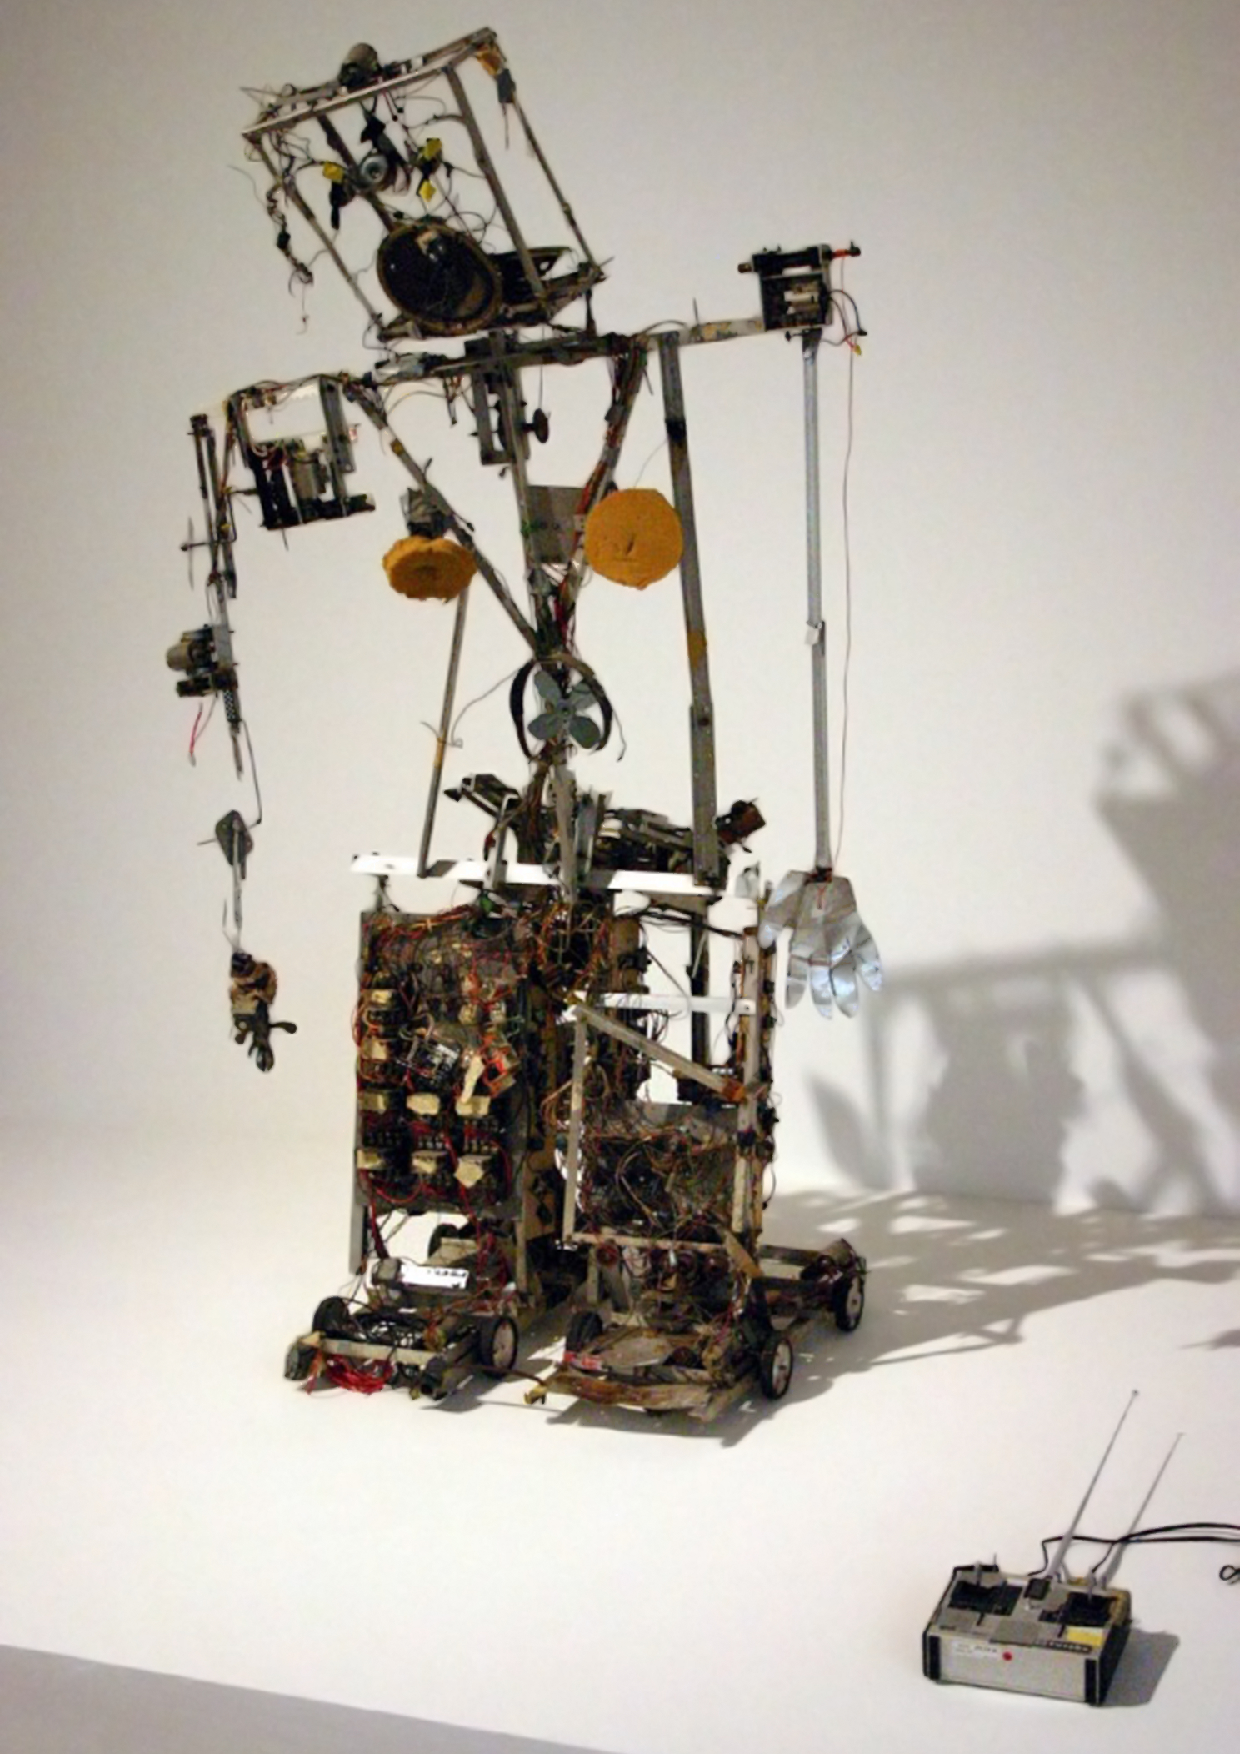
\includepdf{../media/chapter_illustration/Nam_Jun_Paik}

\chapter{Art} % (fold)


\cleanchapterquote{Artists and mathematicians have finally a lot of point in common in the way of working. There is this important role for the mathematician and scientists generally, of inspiration, culture, exchange of ideas, school of thought which change over time or which vary from one country to another, and at the same time, the scientific universality is the same as those found in the arts.}{Cédric Villani}


\section{Introduction} % (fold)

For ages, Science and Art have been mingled. Leonard da Vinci\footnote{Humanist artist who lived during the Renaissance, Leonardo da Vinci had different hat. He was a painter, sculptor and musician but also an engineer, mathematician, physicist, biologist, astrologer, architect and urban planner. Famous today for his painting, he also left visionary flying and war machines.} is a meaningful example of the very existence of such scientific-artist status. Contrary to popular opinion, the two worlds are more agree with each other than opposed. Indeed, in both areas if the methods of investigation and processes implemented to experiment the world may differ, both artists and scientists are motivated toward the same goal: to understand the world around them to share and exchange knowledge with others.

Art often uses results and technology coming from Science applications. These ones are transformed into material resources, instrumental, and technical processes. The example of Futurist\footnote{At the Futurist time, Art seeks to express the dynamism of modern life and the representation of contemporary society: they consider the movement and speed as the most significant emerging phenomena of the twentieth century.} using chronophotography clearly expresses the contribution of science to art. This technique invented by Etienne Jules Marey and Eadweard Muybridge to study human and animal locomotion (see \figurename~\ref{fig:marey_chronophotography}) has been a source of inspiration for Futurists who reproduce in their work the movement decomposition visible in chronophotographies (see \figurename~\ref{fig:duchamp_chronophotography} and \figurename~\ref{fig:russolo_chronophotography}).

\begin{figure}[]
\centering
    \subfloat[][]{\label{fig:marey_chronophotography}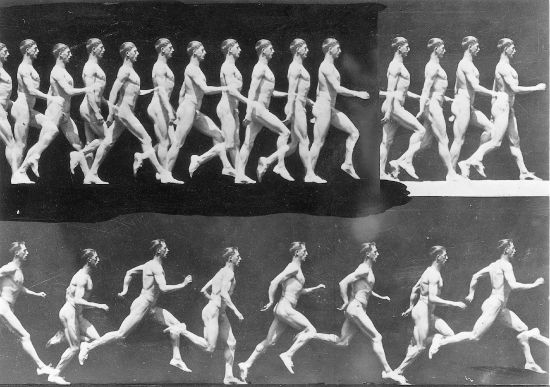
\includegraphics[width=0.8\linewidth]{chronophotography.jpg}}\\
    \subfloat[][Marcel Duchamp, \emph{Nu descendant un escalier}, oil on canvas, 146 x 89 cm (1912) - Philadelphia Museum of Art, Philadelphie (États-Unis).]{\label{fig:duchamp_chronophotography}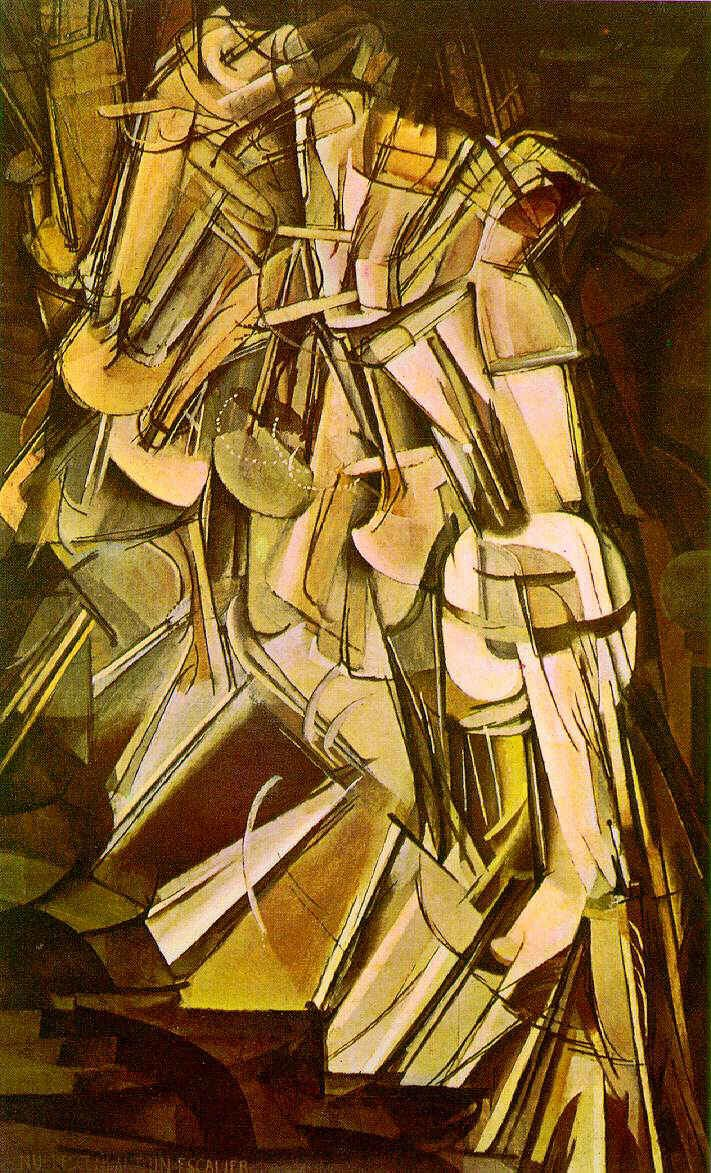
\includegraphics[height=6cm]{chronophotography_duchamp.jpg}}
    \hfil
    \subfloat[][Luigi Russolo, \emph{Dynamisme d’une automobile}, 1912 – Centre Georges Pompidou.]{\label{fig:russolo_chronophotography}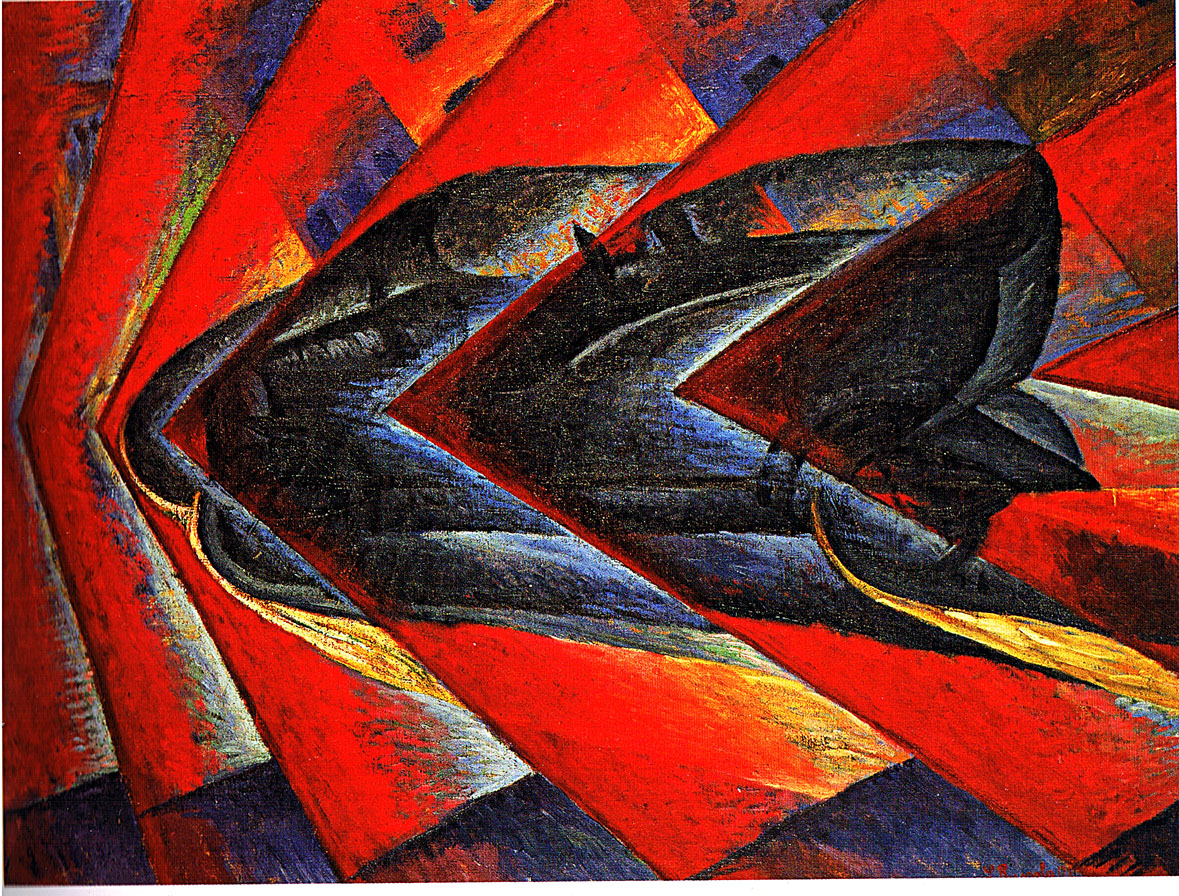
\includegraphics[height=6cm]{chronophotography_russolo.jpg}}
    \caption{}
    \label{fig:chronophotography_history}
\end{figure}

While Science proves to be a source of inspiration for Art, in return, Art is also involved in Science. Some mutations of human thought began first by the arts before spreading to other areas, including scientific; Renaissance is one example among others. In this example, the art in science is manifested through the use of techniques artists by scientists processes. During the Renaissance, the process of molding wax internal cavities used by anatomists was first a process belonging to the art world to be transferred subsequently in the field of science.

Although historically tangible, initiatives involving the 2 worlds are still too few of them. In 1960, C.P.Snow explained in "two culture" theory (REF) that people in humanities and art, and those in the science had developed a sufficiently different language and world-views that they did not understand each other. However, there are actually

In this direction, the Flowers team in collaboration with the artist and movie-maker David Lynch leads a project called "ergo robots" (see \figurename~\ref{fig:ergo_robot}) whose context is the "Mathematics: A Beautiful Elsewhere"\footnote{Mathematics: A Beautiful Elsewhere is a unique exhibition created by the Fondation Cartier pour l’art contemporain with the aim of offering visitors, to use the mathematician Alexandre Grothendieck’s expression, “a sudden change of scenery.” The Fondation Cartier has opened its doors to the community of mathematicians and invited a number of artists to accompany them. They are the artisans and thinkers, the explorers and builders of this exhibition. More info on \url{http://fondation.cartier.com/en/art-contemporain/26/exhibitions/294/all-the-exhibitions/89/mathematics-a-beautiful-elsewhere/}} exhibition in 2011 at the Cartier Foundation for Contemporary Art. The experience of the Flowers team addressing the artificial curiosity, the embodiment and discovery of language in robots, aimed among other goals, the interaction with a non-science-enthusiast public. In this experiment the collaboration between science and art has revealed the art as a medium and tool for scientific mediation.


% \begin{figure}[tb]
%     \begin{center}
%         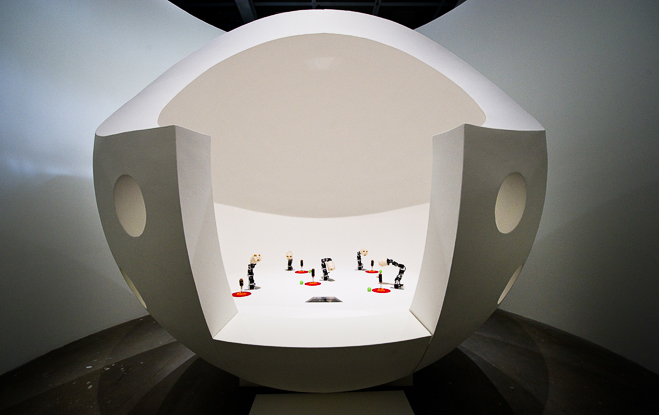
\includegraphics[width=0.8\linewidth]{ErgoRobotFondationCartier.jpg}
%     \end{center}
%     \caption{Caption here}
%     \label{fig:figure1}
% \end{figure}

\begin{figure}[]
\centering
    \subfloat[][]{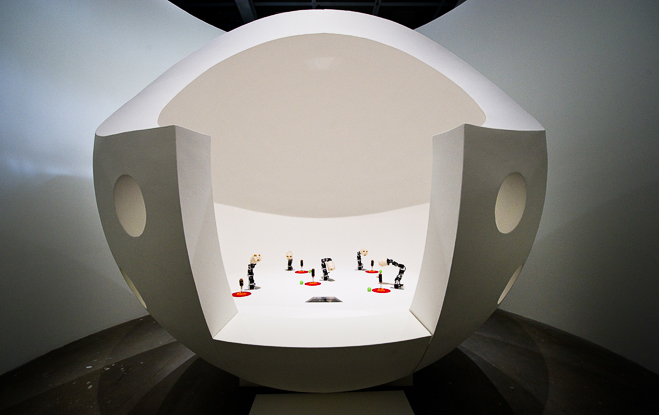
\includegraphics[height=4.2cm]{ErgoRobotFondationCartier.jpg}}
    \hfil
    \subfloat[][]{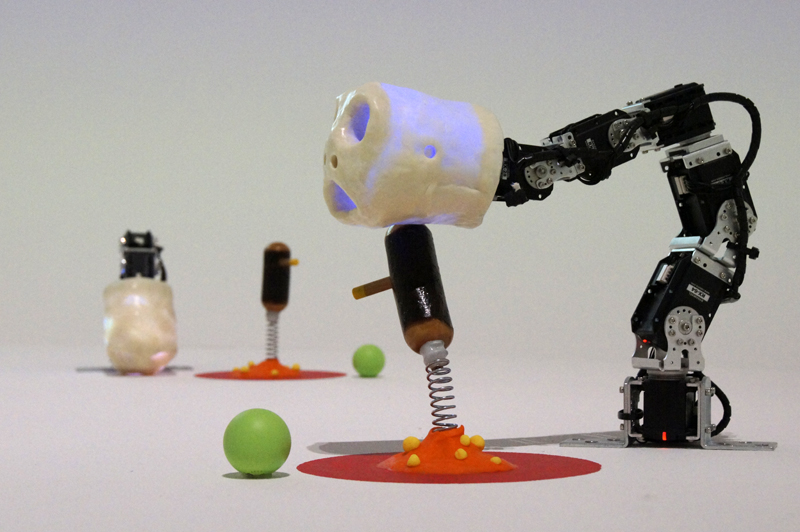
\includegraphics[height=4.2cm]{ErgoRobots13.jpg}}
    \caption{}
    \label{fig:ergo_robot}
\end{figure}

In addition to highlight three of the main fundamental concepts explored in the Flowers team research, going outside the lab raises new and unusual challenges for a research team. Indeed, ergo-robots had to be functional for 5 months 8h/day. Our technologies are really confronted for long term experiences to the real world. In particular, the feedback we get from this experience greatly contribute in the methodology we have built for the design of Poppy.


As we discussed previously, the artist community is a rich source of inspiration and can provide new perspectives to scientific and technological questions. This complementarity is a great opportunity that we want to enforce in the Poppy project by making the robot accessible to non-robotic-expert users.

While it is a real desire to make Poppy accessible and useful for the Art community, we needed to get experience of such uses in an actual artistic project to evaluate how relevant Poppy is for artists and what artists can bring into the Poppy project development.

\section{The \emph{Êtres et numérique} project} % (fold)

The first artistic project in which Poppy is involved is entitled "Êtres et Numérique". This contemporary art project focuses on the way to represent and interact with the movement digitally. It is led by the artists\footnote{Comacina Capsule Creative, \url{http://www.comacina.org/}} Amandine Braconnier (mixed media artist) and Marie-Aline Villard (dancer-researcher), and supervised by Thomas Desmaison (Point barre\footnote{\url{http://www.pointbarre.biz/}}) from the Fabrik Pola\footnote{\url{http://www.pola.fr/}}.

\textbf{A video trailer is available here: \url{https://vimeo.com/92281019}.}

For these artists, the use of an hackable humanoid robot is a whole new expressive tool opening new horizons. Indeed, a robot permits to dissect and analyze movements. It permits to play with its body and model motions as one could sculpt shape in clay. Also, the use of non-rigid actuation allows the emergence of unpredictable and unexpected movement while the fact Poppy is under-actuated ensures safe physical interaction.


The first "Êtres et Numérique" work took the form of a ten days art-science-mediation residency involving members of the Poppy project, the artists with the participation of Jean Marc Weber (music composer) and was supported by the Aquitaine Région. It took place in a Bordeaux(Fr) high school (Lycée Saintonge Sainte Famille\footnote{\url{http://www.lyceesaintefamille.com/}}) which offers its gorgeous chapel (see \figurename~\ref{fig:saintonge_chapel}) for art performances.

\begin{figure}[t]
    \begin{center}
        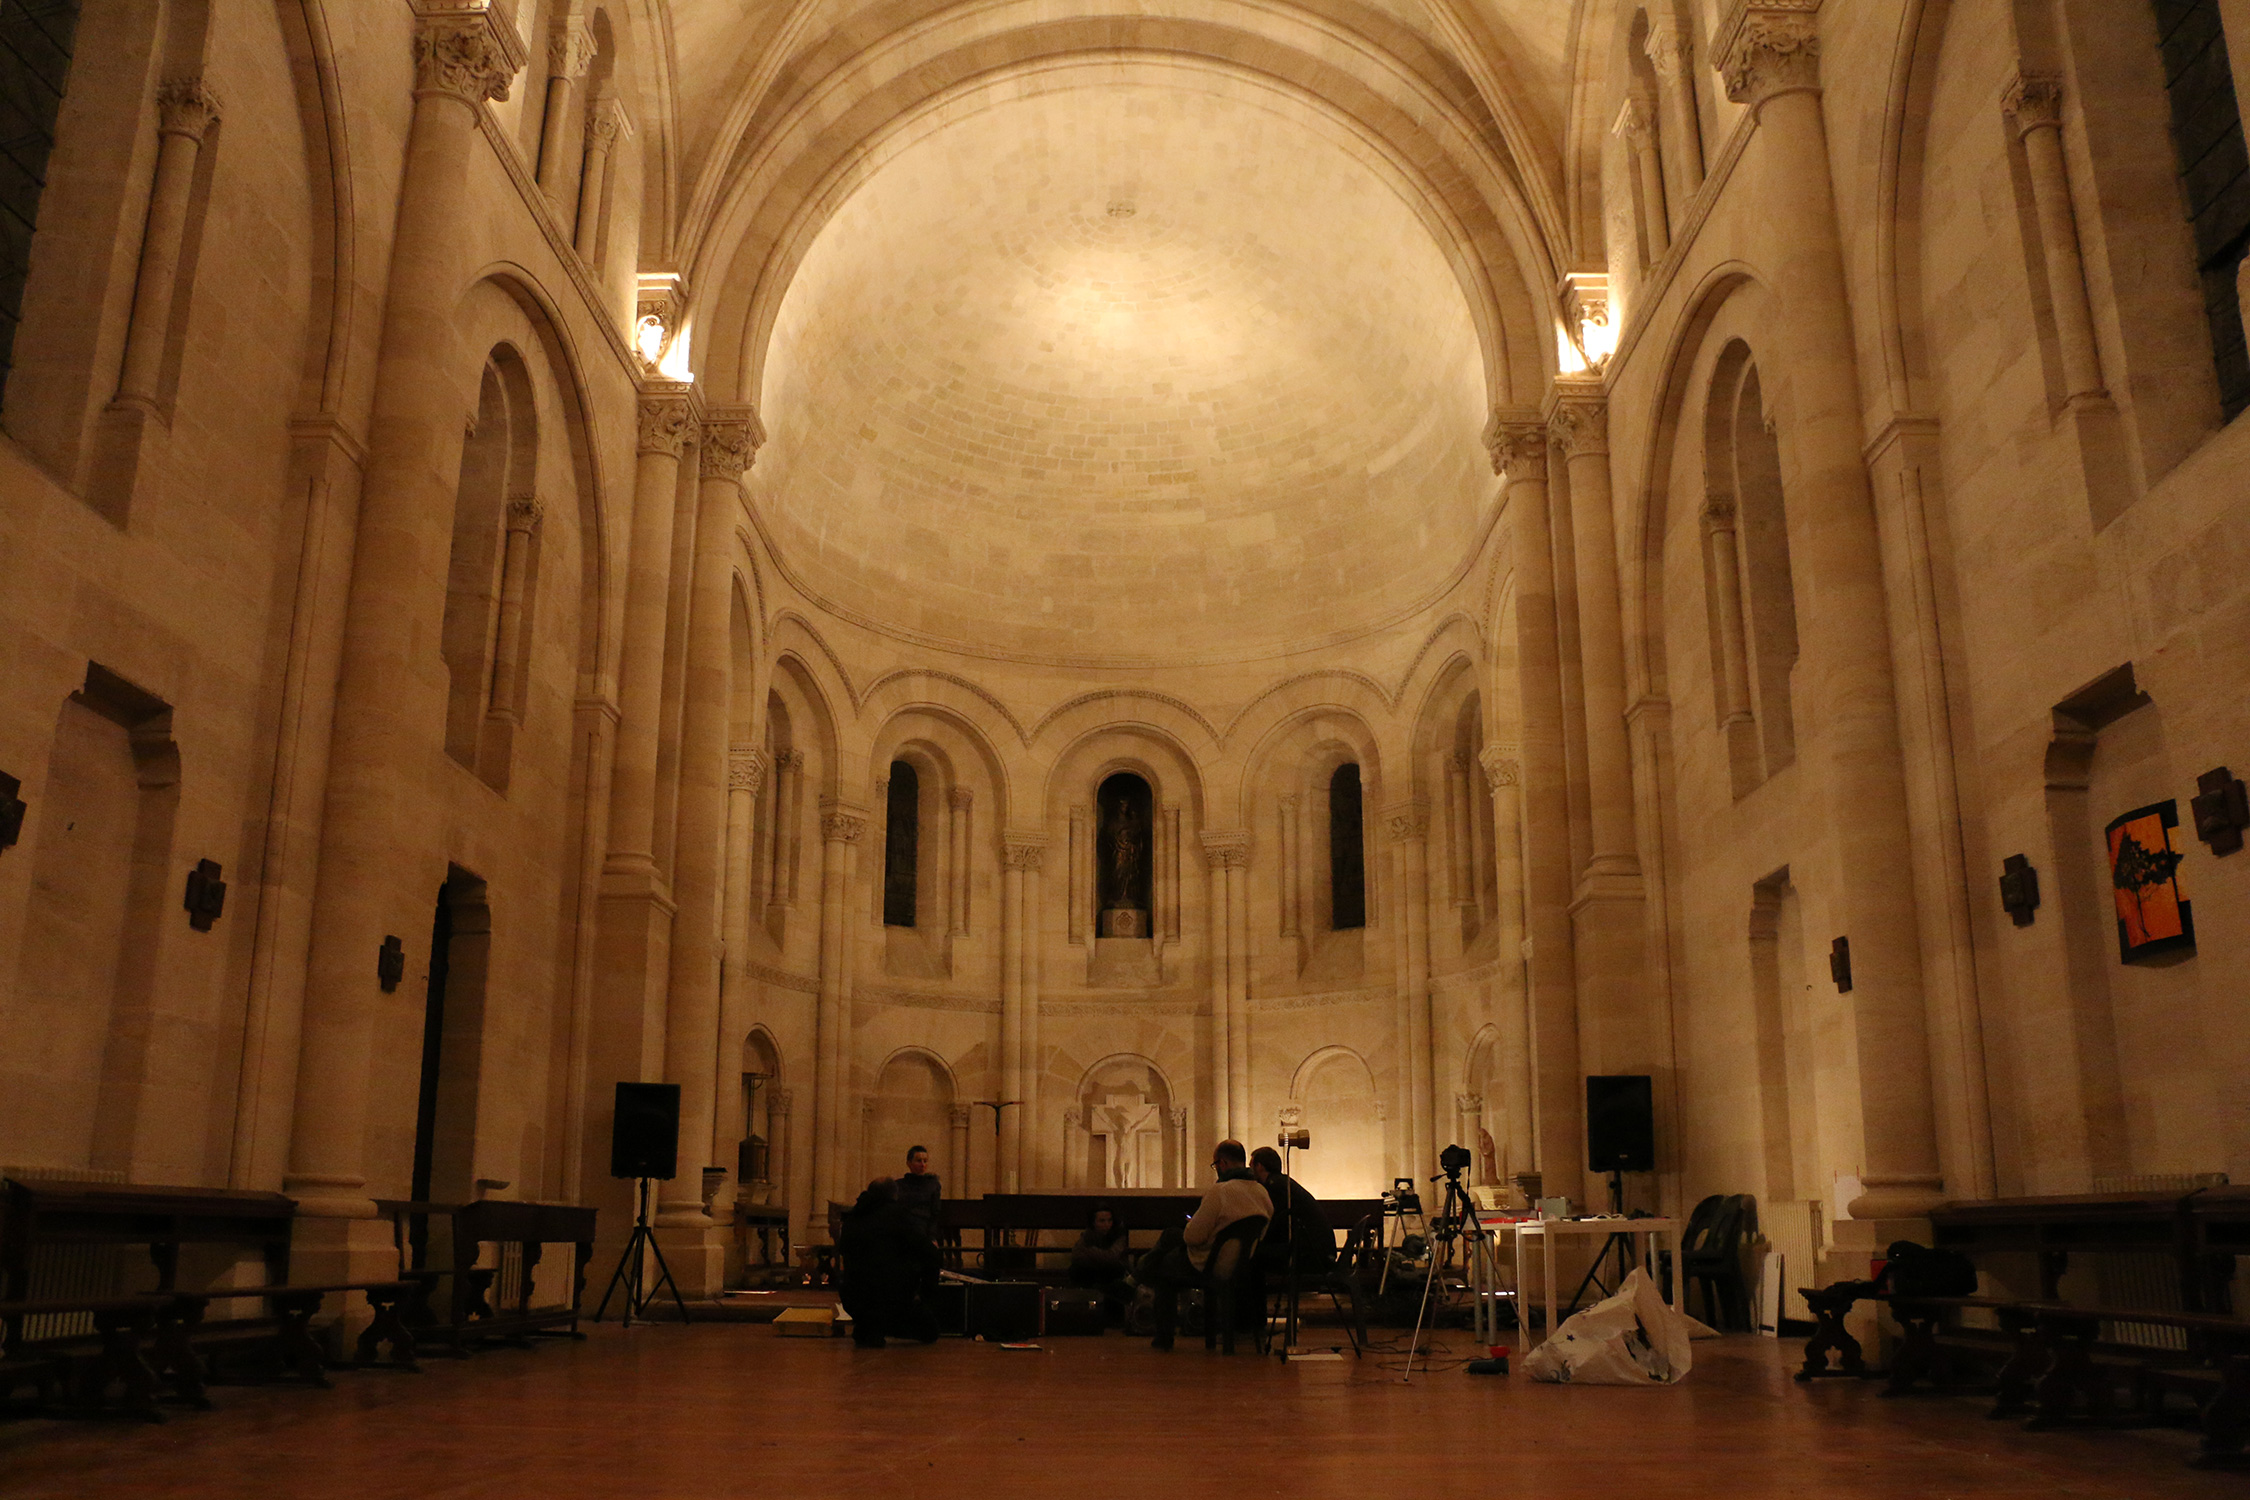
\includegraphics[width=0.8\linewidth]{saintonge_chapel.jpg}
    \end{center}
    \caption{The "Êtres et numérique" residency and performances took place in the gorgeous chapel of the \emph{lycée des metiers Sainte Famille Saintonge}}
    \label{fig:saintonge_chapel}
\end{figure}


This residency was really important for the poppy project: it was the first trial of a real artistic application with Poppy raising new potential applications and bugs.

The main objective of this first residency was the preparation of a dance performance using passive properties of Poppy and physical human-robot interaction with the dancer.


The residency has been organized along three phase:

\begin{itemize}
    \item Exploration with Poppy around several workshop
    \item Master class with students of the high schools where they can participate in th workshop
    \item The end of residency with a dance performance and the exposition of the work done during the residency.
\end{itemize}


\subsection{Artistic exploration} % (fold)

The residency week was an exploring playground for us and Poppy. Several activities took place in parallel with the preparation of the dance performance.

One of the first artistic work was the creation of a canvas series representing in an abstract way the movement combined of the dancer and the robot (see \figurename~\ref{fig:residency_canvas}).

To do so, we dressed Poppy to protect it against dirt (see \figurename~\ref{fig:poppy_dressed}). Then M.A Villard danced with Poppy on canvas covered with pigments (see \figurename~\ref{fig:poppy_playing_with_pigment}). These dancing movements have been captured by pigment traces and have created kind of paintings (see \figurename~\ref{fig:pigment_traces}). The whole collection as been exposed in the chapel (see \figurename~\ref{fig:whole_canvas_collection}.

\begin{NFfigure}
\centering
    \subfloat[][Poppy dressed to protect it against dirt]{\label{fig:poppy_dressed}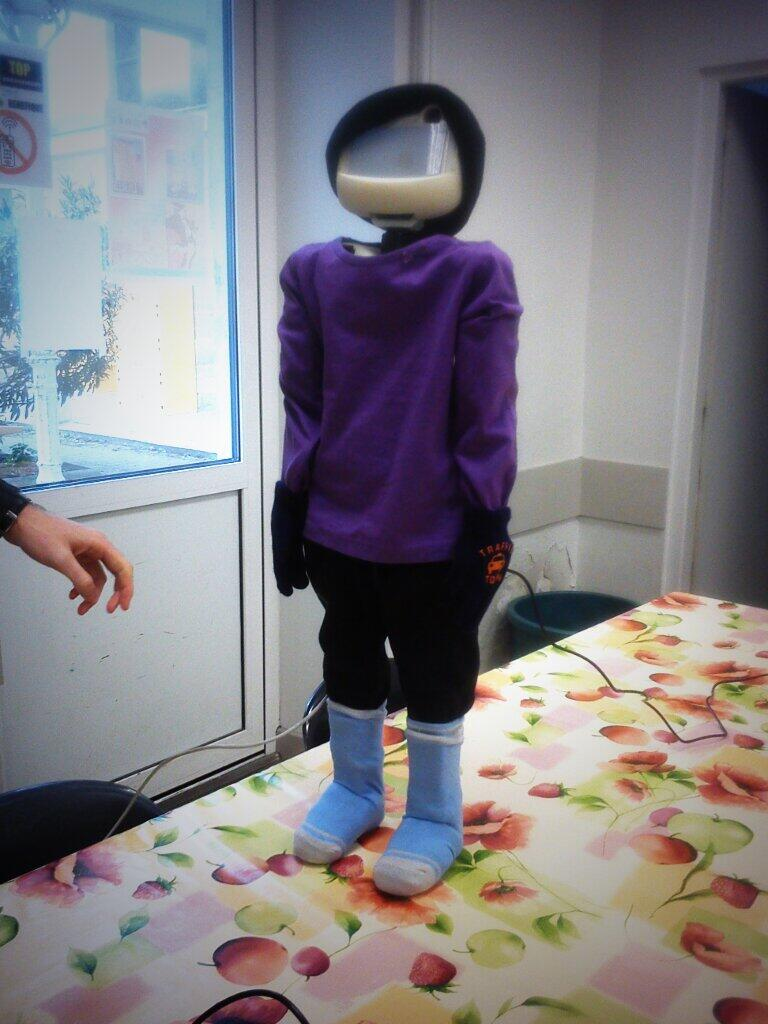
\includegraphics[height=6cm]{poppy_4ans.jpg}}
    \hfil
    \subfloat[][Poppy and the dancer playing on canvas covered with pigments]{\label{fig:poppy_playing_with_pigment}\includegraphics[height=6cm]{IMG_0191.jpg}}\\
    \subfloat[][Result of this human-robot interaction]{\label{fig:pigment_traces}\includegraphics[height=6cm]{_MG_7996.jpg}}
    \hfil
    \subfloat[][The whole canvas collection has been exposed in the chapel]{\label{fig:whole_canvas_collection}\includegraphics[height=6cm]{IMG_0518.jpg}}
    \caption{Movement }
    \label{fig:residency_canvas}
\end{NFfigure}


An alternative way to represent movements can be the use of music produced thanks to motion capture device. This is the playground of Jean Marc Weber, an electro-acoustician and music-composer, creating music using the interaction between probabilistic composer and body space motions. To do so, he created plugins allowing the use of webcam, Kinect or Leap motion with the music-software Usine\footnote{usine TODO}.

These installation were set up to track

TODO

For the dance performance, the dancer's body was tracked using Kinect and sound was associated to each of

At the beginning, we only though we will track the dancer and create music but we were curious about the

When Poppy is dressed it can definitely be tracked by Kinect sensor\footnote{A video was taken during tests and is accessible here: \url{https://www.youtube.com/watch?v=VVjBVTtPkFE}}, also thanks to its hands using human shape, it can also play with the Leap motion (see \figurename~\ref{fig:poppy_playing_leap}).

\begin{NFfigure}
\centering
    \subfloat[][Poppy playing music with Leap motion device]{\label{fig:poppy_playing_leap}\includegraphics[height=6cm]{IMG_0049.jpg}}
    \hfil
    \subfloat[][Poppy playing music with Kinect]{\label{fig:poppy_playing_kinect}\includegraphics[height=6cm]{IMG_0258.jpg}}
    % \subfloat[][Poppy and the]{\label{fig:}\includegraphics[height=4.5cm]{IMG_0434.jpg}}
    \caption{}
    \label{fig:}
\end{NFfigure}

Amandine Braconier (Plastic artist) wanted to make an experiment with a little child (3 years). In this experiment, the child can modify the robot appearance by adding clay on it (see \figurename~\ref{fig:clay_on_poppy}). To protect Poppy, we wrapped it with cellophane.

This experiment last about 2h and the clay is really heavy. It turns out to be playful for the little boy to put as much clay as possible. Eventually he managed to put almost 10kg on the poor Poppy\dots

\begin{NFfigure}
\centering
    % \subfloat[][Poppy covered with cellophane ready to be modify using clay]{\includegraphics[height=3cm]{IMG_0379.jpg}}
    % \hfil
    \subfloat[][Poppy covered with cellophane ready to be modify using clay]{\includegraphics[width=0.49\linewidth]{IMG_0381.jpg}}
    \hfil
    \subfloat[][Little boy playing while Poppy is silently suffering from all the extra weight put on it.]{\includegraphics[width=0.49\linewidth]{_MG_8034.jpg}}
    \caption{}
    \label{fig:clay_on_poppy}
\end{NFfigure}


\subsection{The dance performance} % (fold)

The residency restitution was a public (about a hundred people) contemporary art dance performance involving poetic choreography, alternating phases of autonomous robot movements and passive robot movements provoked by the dancer (see \figurename~\ref{fig:poppy_dance_performance}).

In particular, using the pypot feature to directly record movements by demonstration, the dancer, M.A. Villard, managed to sculpt a whole floor choreography where Poppy slowly move with elegance and sensibility.

Despite the problems we have had during the residency, Poppy acted really great and no technical problem occurred.The whole dance performance last about 20min and was repeated 4 times in a row without any interruption.

\textbf{A complete performance set can be seen here: \url{http://youtu.be/zp-vsVQcAvs}.}

\begin{figure}[]
\centering
    \subfloat[][]{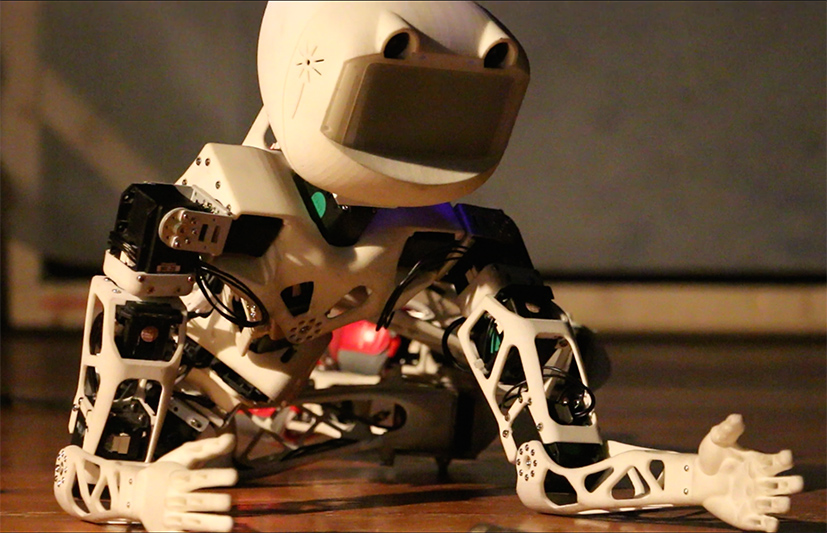
\includegraphics[width=0.46\linewidth]{ENP_img2.png}}
    \hfil
    \subfloat[][]{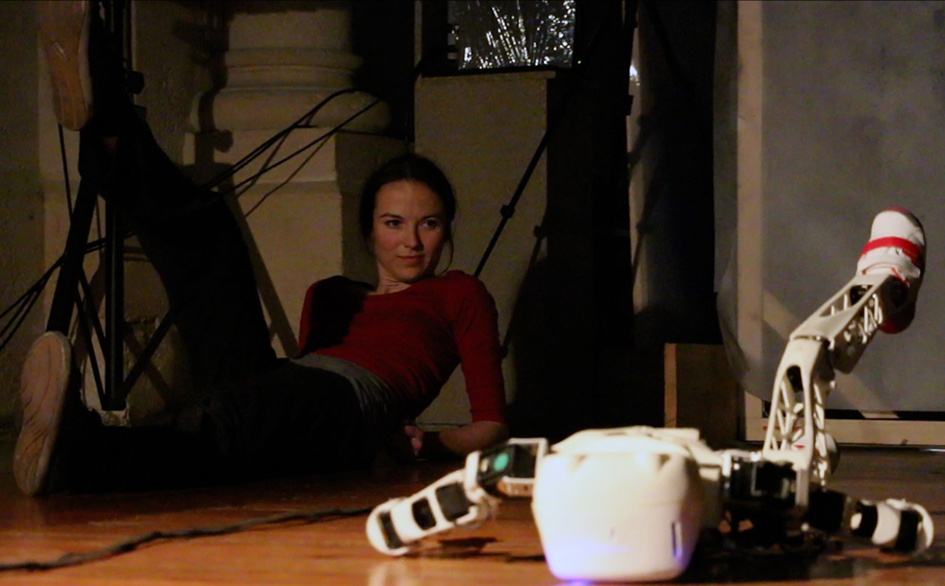
\includegraphics[width=0.46\linewidth]{art_floor.jpg}}\\
    \subfloat[][]{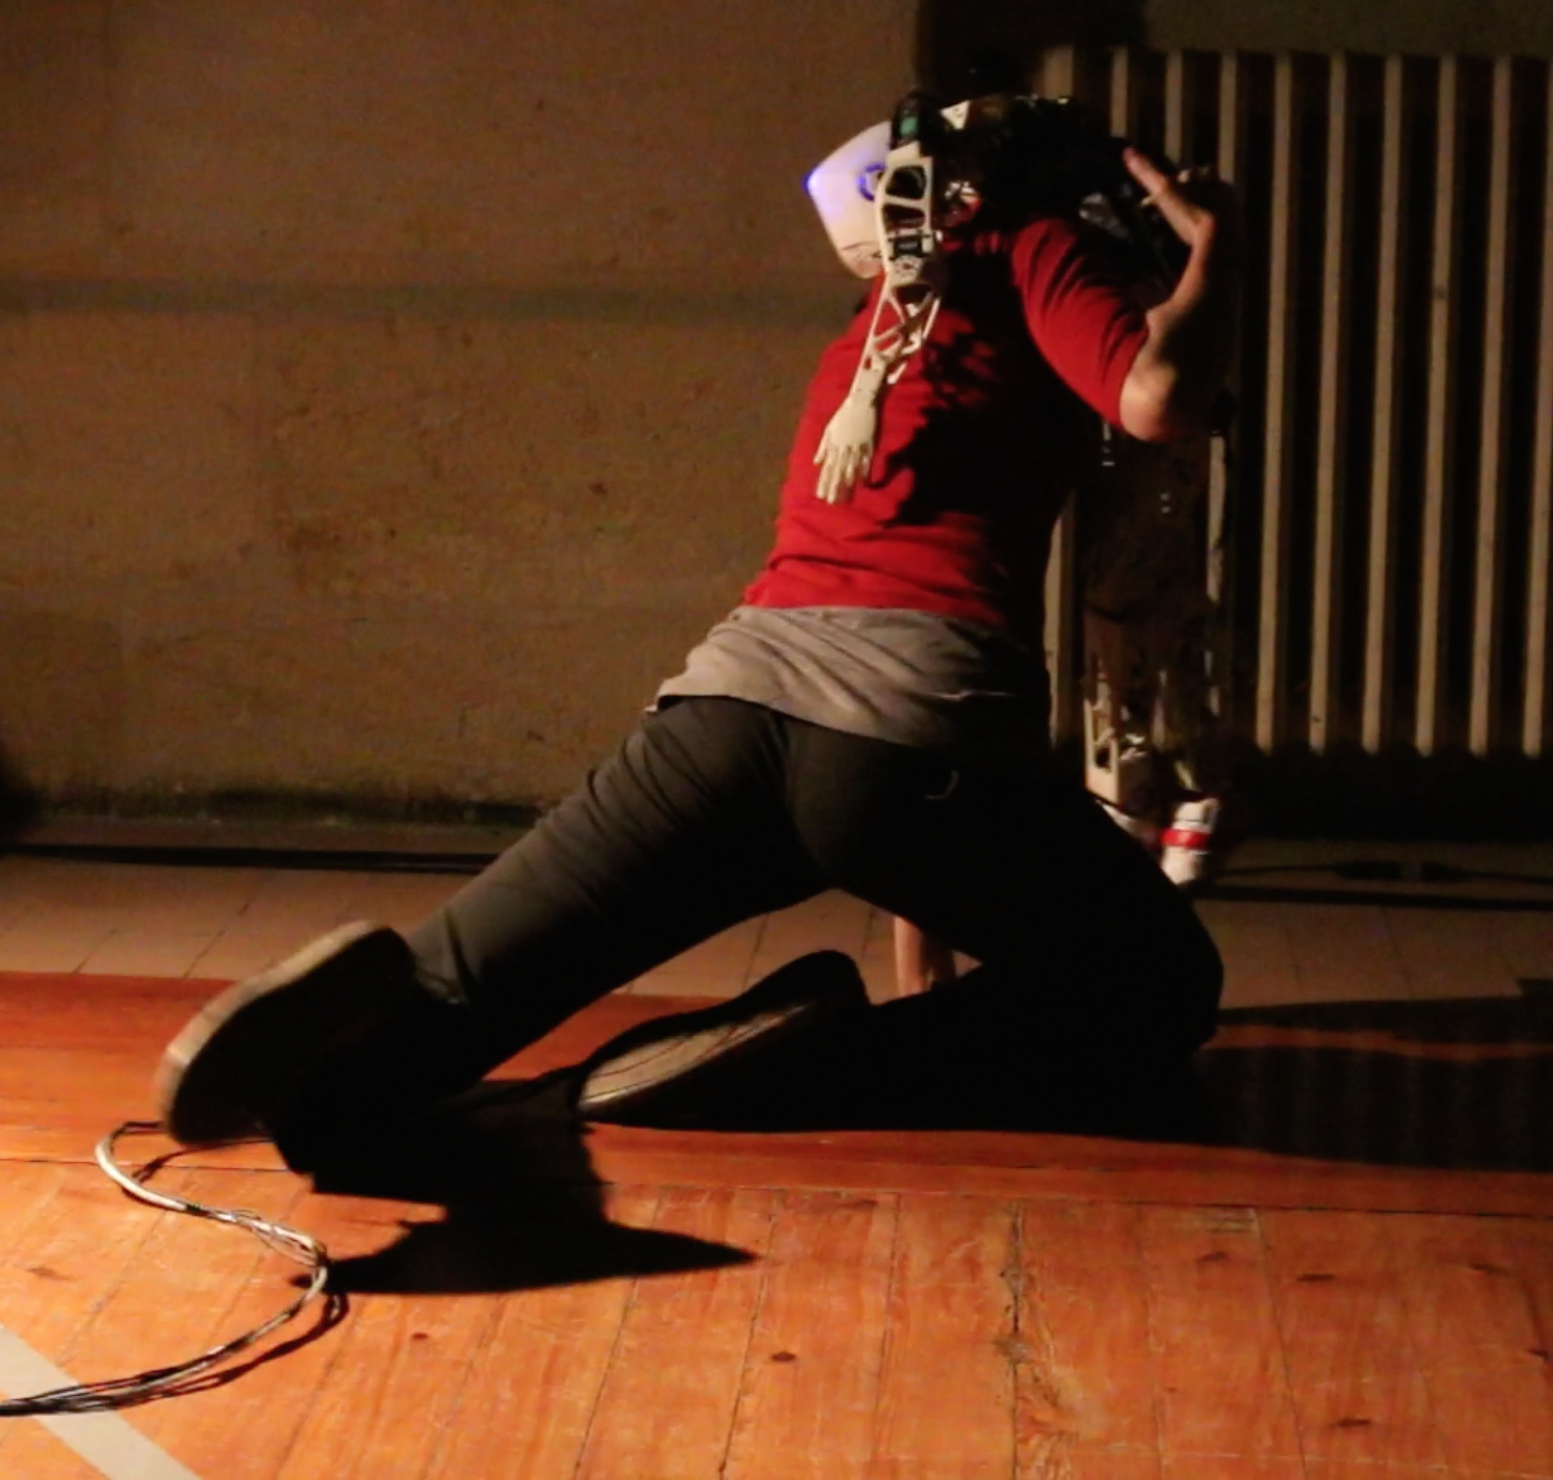
\includegraphics[height=5.3cm]{img6.png}}
    \hfil
    \subfloat[][]{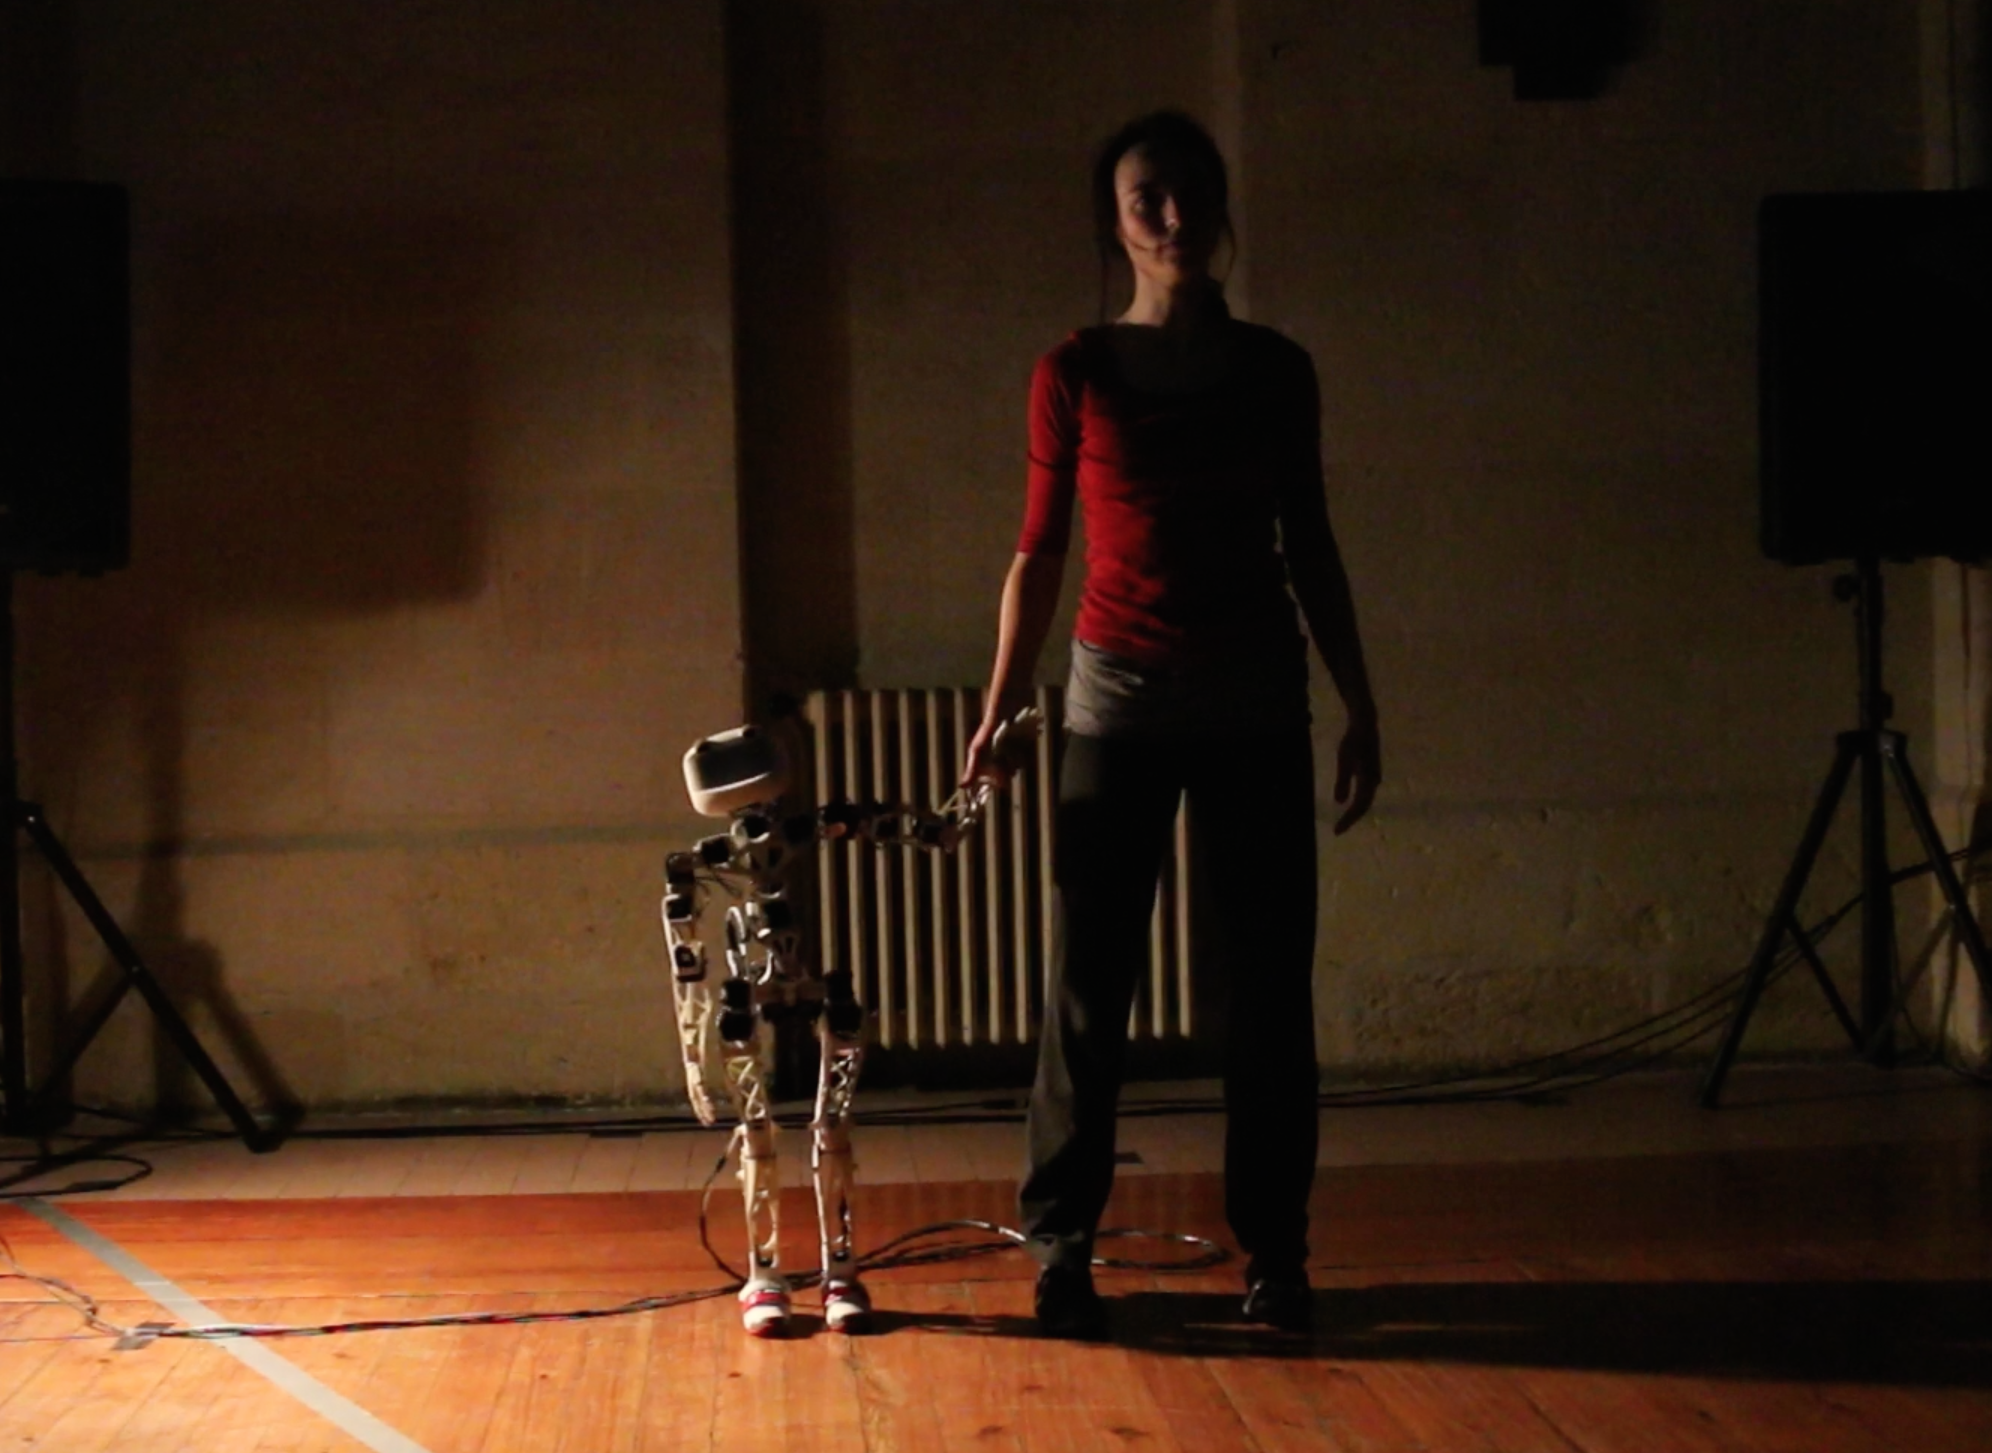
\includegraphics[height=5.3cm]{poppy_dancer_stand_up.png}}\\
    \subfloat[][]{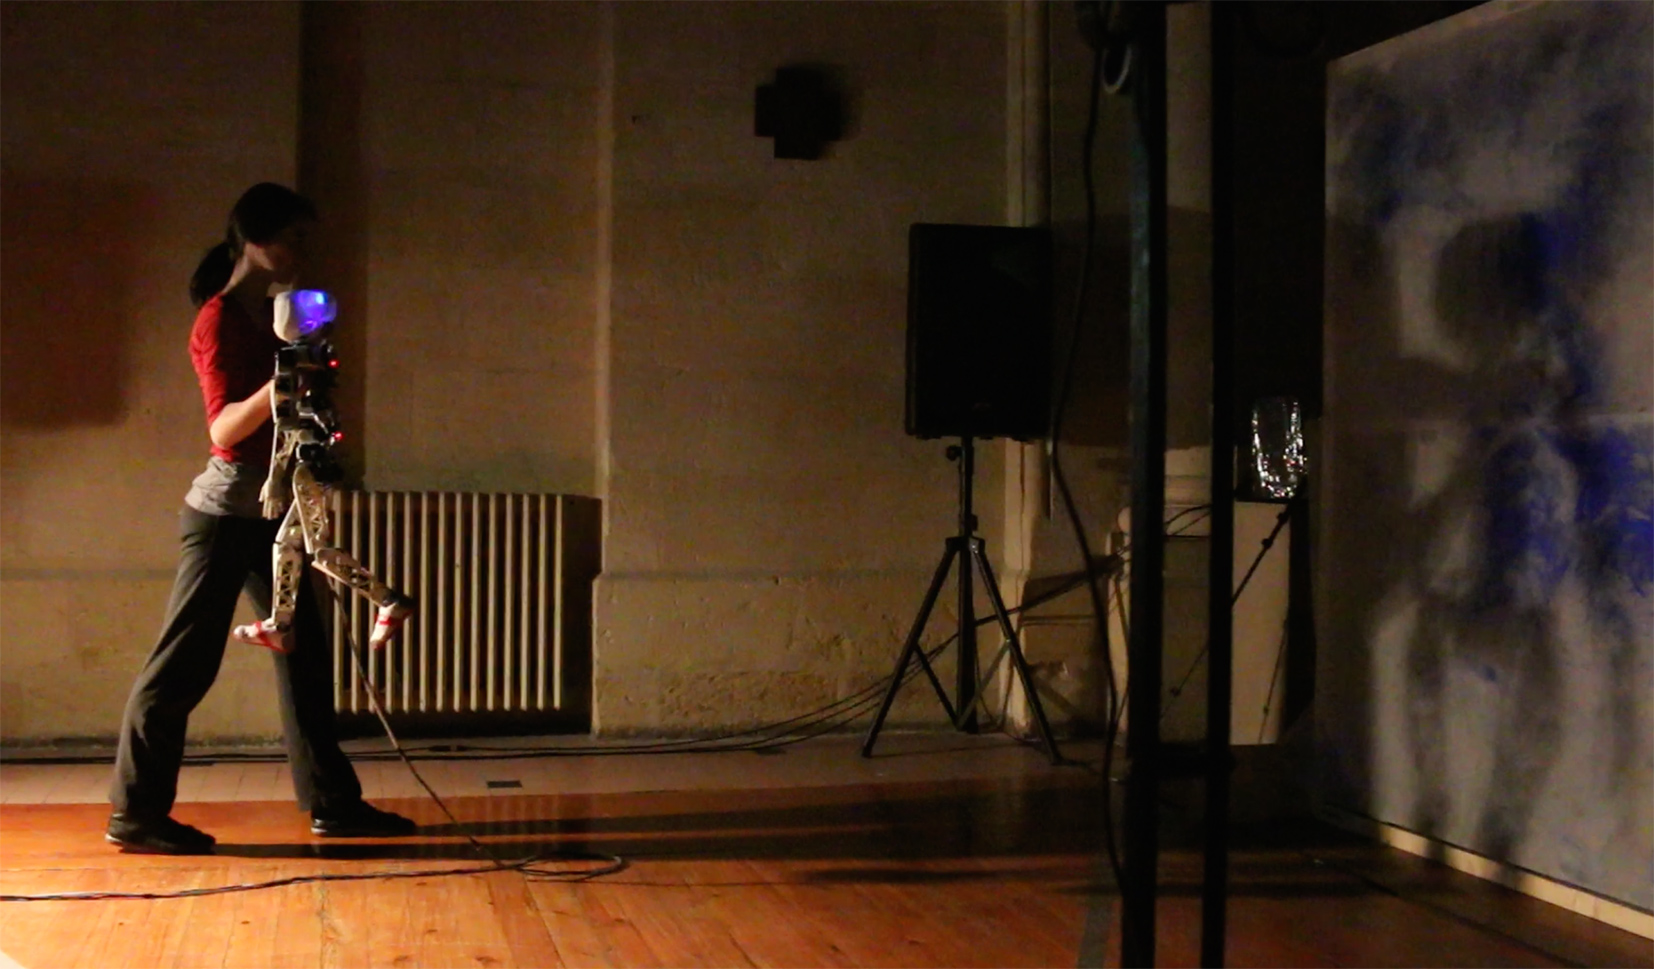
\includegraphics[width=0.95\linewidth]{img3.png}}
    \caption{}
    \label{fig:poppy_dance_performance}
\end{figure}




\subsection{Feedback} % (fold)

% \subsubsection{Problems raised} % (fold)

Unfortunately or fortunately, all these workshops did not occurred without problems with the use of Poppy by artists(\figurename~\ref{fig:broken_poppy_residency}).

First, it appears it is difficult for non-expert user to evaluate the actual resistance of Poppy. After some times acting really preciously with it, they get confident about its robustness and do not pay attention no more to signs indicating the robot is going to be broken. The experience with the little boy putting clay has been quite destructive. Poppy spent almost 2 hours in cellophane supporting kilos of clay, eventually it overheated and two motors in the hip and abs have melted.
Thus it appears really needed to add security system raising alerts when the robot is in a dangerous state.  Otherwise non-expert people will break regularly motors without understanding why.

\begin{figure}[]
\centering
    \subfloat[][]{\includegraphics[height=4.5cm]{IMG_0019.jpg}}
    \hfil
    \subfloat[][]{\includegraphics[height=4.5cm]{IMG_0046.jpg}}
    \caption{}
    \label{fig:broken_poppy_residency}
\end{figure}

Second, the strong interaction between Poppy and the dancer showed it was really complicated, when the robot is compliant, to avoid motors to go on their dead-band. In addition, wires tend to tangling around motors, which eventually unplug some of them. To avoid this recurrent problem, we built a pypot primitive checking the state of each motor and stopping it when it reach a given amplitude. Also, we are working on mechanical way to avoid full-rotation of certain Poppy links.

Third, the wire are really problematic, they caused a lot of problem along the residency. In this context of intensive use of the robot doing large amplitude motion, wires have been solicited and eventually some of them began to be damaged which provoked short-circuit and so destroyed some motors and micro-controller.

During the residency, the ease of programming through the Pypot library permitted to design a simple interface allowing the dancer to physically sculpt novel movements, which softness could be dynamically controlled.

The pypot programing by demonstration is really basic, position are recorded at 50hz and played. It is not at all optimized and yet a bit annoying to use because you cannot edit your moves. But this way to "program" the robot has also a great advantage. The artist really appreciate to sculpt motion like this rather than editing curve on a nice interface because she can really feel the weight of the robot and work on the way to move its mass from one support to another. Finally, because Poppy is not over-actuated, it constrains motion to whom requiring the less power actuation and therefore leads to the creation of more natural motion.


\section{Conclusion} % (fold)
As the Ergo-robots experience, the artist residency around Poppy we had has been really instructive. First, Poppy has been used in totally unknown and unexpected(able) situations, playing in pigments, dancing 2h long and so on were not on the development todo list. It was a real crash test for a novel experimental platform. Again, like in the ergo-robot experience, we learn the hard way how problematic are the wires. Most of the problem we had were due to damaged wires which provoked short-circuit and eventually destroyed some motor and micro-controller. It is a real problem in robotic right now, and it is really complicated to find a way to avoid it while keeping a modular et highly hackable robot.

But beyond the technical aspects, the work the artists did with Poppy was really amazing and they find unexpected potential in Poppy. Among them, the choreography Marie Aline Villard did, was so elegant and sensible. These movements put Poppy in a sensible domaine rarely saw in humanoid robotics. This choreography is now often used for demonstration of the Poppy platform and closes the communication video showing Poppy being assembled in timelapse \url{https://vimeo.com/96262428}.

Also, from a community impact point of view, the topic\footnote{\url{https://forum.poppy-project.org/t/artist-residency-etres-et-numerique/}} related the experience is by far the most followed subject of our forum.

\section{Discussion} % (fold)

\begin{quotation}
    As a dancer, shared this experience with Poppy movement was very interesting on both the artistic and functional/mechanical aspects. On one hand, I liked working on the line between who animates who, trying to give the illusion of a duet. But on the other hand, I am also amused to show that Poppy was still an object by playing on active/passive and by manipulating genuinely. This edge is a great discovery and artistic research should continue in this direction.
    Also sharing the movement with robotic object remains fascinating, since we projects our own movement patterns. I could check during a workshop, at which point we were planning our own move on the structure of the robot. By asking students to make movement between a posuter A and a posture B, in spite of themselves they began moving, dancing, just to record a movement for the robot, which leads me to say that Poppy has disinhibiting properties, to exploit in the interaction and that dance can greatly contribute.

    \signed{Mari-Aline Villard (Dancer) on the use of Poppy for artistic project}
\end{quotation}


\begin{quotation}
    How to use Poppy? The robot is put to the test. I do not know in advance what will happen. Each experiment is photographed and filmed. Some sequences are mounted. I try to emerge from other movements that have not been calculated by the researchers. For example, I suggested an interaction with the robot: a child, through the game, evolves with Poppy. It is in a back and forth continuously between the two actions that the child and the robot meet, separate and detached. In the exchange that occurs remains a singularity and shows a confusion. On the video, we see the child cover the with clay the robot. It transforms it. It gives it a monstrous appearance. Also, the action of the child on the robot causes his downfall. The robot is as if exhausted. We do not know which of the two is the monster. The effect far beyond the game. The aim here is to choose what we will do with Poppy and how we will show it.
    \signed{Amandine Braconier (06/18/2014)}
\end{quotation}





% \section*{sources} % (fold)
% \label{sec:sources}

% % section sources (end)
% Before the renaissance, Art and Science were united. Science was called natural philosphy. Philosopher were as likely to speculate about art and science as about religion and truth. During the renaissance Science became specialized and codified while art moved on its way. With the industrial era, Science inspired Technology and viseversa. Research and invention spread in every day life while Art seemed oblivious. Increasingly, it became lees likely that an educated person will be well-versed in both areas of culture.

% In 1960 commentator CP Snow,developped his influancial "two culture"theory (ref) taht conducted those in humanities and art and those in the science had developed suffienctly differente langaeg and worldviews that they did not undesrtand each other.


% Si le passé, les affinités heuristiques et la réalité de terrain montrent que les arts et les sciences se fréquentent de longue date, force est de constater cependant que leurs relations demeurent trop timides aujourd’hui. Sans doute se sont-elles même distanciées avec la spécialisation croissante des champs du savoir et du faire, chacun se repliant sur son domaine pour défricher ses problématiques et cultiver ses ambitions.


% Ainsi que l'écrit le physicien Léo Szilard[L.Szilard, "Genius in the Shadows", Charles Scribner's Sons, 1992.], "le scientifique créatif a beaucoup en commun avec l'artiste et le poète. Il doit faire preuve de pensée logique et de capacité d'analyse, mais s'est loin d'être suffisant pour faire un travail créatif. Les idées nouvelles qui ont conduit à de grandes percées n'ont pas été déduites logiquement des connaissances préexistantes : les processus créatifs, sur lesquels repose le progrès scientifique, opèrent à un niveau inconscient".

% La science pose en effet les questions fondamentales du vivant. « Jusqu’au 18e siècle, l’art est étroitement lié à la religion, qui porte alors les sujets existentiels. De nos jours, c’est la science qui les pose, ce qui rend la collaboration indispensable pour que l’art continue de traiter des grandes questions de la vie. » note le plasticien Paolo Castagna.


% « La rencontre entre des personnes d'horizons différents affute les regards, construit les conditions d'une vigilance et une forme de don réciproque propice à l'émergence d'idées nouvelles. Les relations humaines deviennent une des conditions première de l'activité de recherche conjointe. La convocation d'un double imaginaire (technique et sociétal) favorise le replacement des activités de recherche au cœur des activités humaines. » pointe  fort justement Antoine Conjard, directeur de L’Hexagone-scène nationale de Meylan.


% les impacts économiques militent aussi pour une collaboration plus étroite. Déjà, en 1998, le rapport Art-Science-Technologie, établi sous la direction de Jean-Claude Risset, soulignait que « Les enjeux économiques de la recherche artistique sont considérables. Les arts alimentent des industries culturelles au marché potentiel très important. Les applications de la recherche en art concernent l'activité artistique professionnelle mais aussi l'éducation et les loisirs. ». Le développement de la créativité artistique et la vitalité économique apparaissent indissociables au fil d’une démonstration fort documentée.


% Puissant stimulant de l’imaginaire, la recherche artistique a d’ailleurs souvent inspiré le travail scientifique et l'innovation technologique. C'est ainsi par l’observation de phénomènes musicaux que Pythagore a appliqué l'arithmétique à l'étude des phénomènes naturels. L’histoire de la musique fournit bien d’autres exemples, notamment avec l’informatique musicale, développée à l’instigation de compositeurs, qui a donné d’importantes innovations dans d’autres domaines, tels que le calcul ou l’acoustique architecturale. « Dans les années 1950, le musicien Yannis Xenakis imaginait avant les scientifiques, les développements de l'électronique dans les arts du signe et du son. Plus tard, dans les années 70/80, la 4X, une machine de synthèse de son conçue à l’IRCAM sur spécifications de compositeurs tels que Luciano Berio, fut la machine de calcul la plus puissante en France. A tel point que SOGITEC en acheta deux pour réaliser des simulateurs de vol pour les militaires, raconte Dominique David, chercheur en traitement de l’information au CEA de Grenoble. Encore aujourd’hui, la reconnaissance gestuelle mise au point par l’IRCAM est au moins une des plus abouties, si ce n’est la plus aboutie. »



% En se mêlant à la création artistique, la science et ses applications techniques trouvent également un vecteur original de médiation pour atteindre le public non initié. L’expérience sensible qu’appelle une œuvre d’art favorise l'appropriation des technologies innovantes ou les résultats de recherches, notamment parce qu’elle démystifie la complexité des mécanismes mis en jeu grâce à une approche sensorielle et une production concrète, plus aisément appréhendable que des explications théoriques. Ce faisant, elle permet souvent d’en comprendre les enjeux, les utilisations potentielles, de désamorcer des craintes liées à leur nouveauté et d’élargir leur diffusion.

